% =====================================================================
% 04_bezier.tex  --  Bezier Curves, Bezier Surfaces, De Casteljau
% Bilingual EN | VI cheatsheet section for IT516 Advanced Computer Graphics
% =====================================================================

\section*{4.\ Bezier Curves, Bezier Surfaces, De Casteljau \;|\; \textit{Đường cong, Mặt Bezier, Thuật toán De Casteljau}}

\begin{paracol}{2}

% ---------------------------------------------------------------------
% 4.1  DEFINITION & BERNSTEIN FORM
% ---------------------------------------------------------------------
\subsection*{4.1 Bezier Curve --- Bernstein Form}

A \textbf{Bezier curve} of degree $n$ with $n{+}1$ control points $P_0,\dots,P_n$ is the parametric curve
\[
B(t)=\sum_{i=0}^{n}\binom{n}{i}(1-t)^{\,n-i}t^{\,i}P_i,\quad t\in[0,1].
\]
The polynomials
\[
B_i^{\,n}(t)=\binom{n}{i}(1-t)^{\,n-i}t^{\,i},\quad i=0,\dots,n
\]
are called \textbf{Bernstein basis polynomials}.

\textbf{Key properties.}
\begin{itemize}[leftmargin=*,nosep]
  \item \emph{Endpoint interpolation:} $B(0)=P_0,\ B(1)=P_n$.
  \item \emph{Partition of unity:} $\sum_{i=0}^{n}B_i^{\,n}(t)=1$ for all $t$ $\Rightarrow$ \emph{affine invariance}.
  \item \emph{Convex hull:} $B(t)\in\operatorname{conv}\{P_0,\dots,P_n\}$ since $B_i^{\,n}(t)\ge 0$.
  \item \emph{Variation diminishing:} the curve crosses any line/plane no more times than its control polygon does $\Rightarrow$ no extra wiggles.
  \item \emph{Symmetry:} $B(t)$ with control points reversed equals $B(1{-}t)$, i.e.\ $B_i^{\,n}(t)=B_{n-i}^{\,n}(1-t)$.
  \item \emph{Endpoint tangents:}
        $B'(0)=n(P_1-P_0),\ B'(1)=n(P_n-P_{n-1})$.
  \item \emph{Pseudo-local control:} moving $P_i$ shifts $B(t)$ proportionally to $B_i^{\,n}(t)$ (max at $t=i/n$).
  \item \emph{Degree:} a Bezier curve with $n{+}1$ points is a polynomial of degree $\le n$.
\end{itemize}

\switchcolumn

\subsection*{4.1 Đường cong Bezier --- Dạng Bernstein}

\textbf{Đường cong Bezier} bậc $n$ với $n{+}1$ control point $P_0,\dots,P_n$ là đường cong tham số
\[
B(t)=\sum_{i=0}^{n}\binom{n}{i}(1-t)^{\,n-i}t^{\,i}P_i,\quad t\in[0,1].
\]
Các đa thức $B_i^{\,n}(t)=\binom{n}{i}(1-t)^{\,n-i}t^{\,i}$ gọi là \textbf{đa thức cơ sở Bernstein}.

\textbf{Tính chất quan trọng.}
\begin{itemize}[leftmargin=*,nosep]
  \item \emph{Nội suy đầu mút:} $B(0)=P_0,\ B(1)=P_n$.
  \item \emph{Tổng bằng 1:} $\sum B_i^{\,n}(t)=1$ $\Rightarrow$ \emph{bất biến affine} (xoay/tịnh tiến control point thì curve cũng biến đổi tương ứng).
  \item \emph{Bao lồi:} đường cong luôn nằm trong bao lồi của các control point.
  \item \emph{Giảm dao động (variation diminishing):} đường cong cắt một đường thẳng không nhiều hơn số lần control polygon cắt đường đó.
  \item \emph{Đối xứng:} đảo thứ tự control point thì $B(t)$ trở thành $B(1{-}t)$.
  \item \emph{Tiếp tuyến tại đầu mút:}
        $B'(0)=n(P_1-P_0)$, $B'(1)=n(P_n-P_{n-1})$.
  \item \emph{Điều khiển gần địa phương:} khi dời $P_i$, curve dịch chuyển nhiều nhất tại $t=i/n$.
  \item \emph{Bậc:} curve là đa thức bậc $\le n$.
\end{itemize}

\switchcolumn*

% ---------------------------------------------------------------------
% 4.2  SPECIFIC CASES
% ---------------------------------------------------------------------
\subsection*{4.2 Specific Low Degrees}

\textbf{Linear} ($n=1$, $P_0,P_1$):
\[
B(t)=(1-t)P_0+tP_1.
\]
\textbf{Quadratic} ($n=2$, $P_0,P_1,P_2$):
\[
B(t)=(1-t)^{2}P_0+2(1-t)tP_1+t^{2}P_2.
\]
\textbf{Cubic} ($n=3$, $P_0,P_1,P_2,P_3$) -- the most-used in graphics:
\[
B(t)=(1-t)^{3}P_0+3(1-t)^{2}tP_1+3(1-t)t^{2}P_2+t^{3}P_3.
\]
\textbf{Quartic} ($n=4$):
\[
B(t)=\sum_{i=0}^{4}\binom{4}{i}(1-t)^{4-i}t^{\,i}P_i.
\]

\textbf{Pascal's triangle} (binomial coefficients):
\begin{center}\small
\begin{tabular}{c|ccccccc}
$n$ & & & & coefficients & & & \\\midrule
0 & & & & 1 & & & \\
1 & & & 1 & & 1 & & \\
2 & & & 1 & 2 & 1 & & \\
3 & & 1 & 3 & 3 & 1 & & \\
4 & 1 & 4 & 6 & 4 & 1 & & \\
5 & 1 & 5 & 10 & 10 & 5 & 1 & \\
\end{tabular}
\end{center}

\switchcolumn

\subsection*{4.2 Một số bậc thường gặp}

\textbf{Tuyến tính} ($n=1$): $B(t)=(1-t)P_0+tP_1$ -- chính là phép nội suy tuyến tính giữa hai điểm.

\textbf{Bậc hai} ($n=2$):
$B(t)=(1-t)^{2}P_0+2(1-t)tP_1+t^{2}P_2$.

\textbf{Bậc ba} ($n=3$) -- thông dụng nhất trong đồ hoạ và font chữ:
$B(t)=(1-t)^{3}P_0+3(1-t)^{2}tP_1+3(1-t)t^{2}P_2+t^{3}P_3$.

\textbf{Bậc bốn} ($n=4$): tương tự, hệ số $\binom{4}{i}=1,4,6,4,1$.

\textbf{Tam giác Pascal} dùng để tra hệ số nhị thức $\binom{n}{i}$:
\begin{center}\small
\begin{tabular}{c|ccccccc}
$n$ & & & & hệ số & & & \\\midrule
0 & & & & 1 & & & \\
1 & & & 1 & & 1 & & \\
2 & & & 1 & 2 & 1 & & \\
3 & & 1 & 3 & 3 & 1 & & \\
4 & 1 & 4 & 6 & 4 & 1 & & \\
5 & 1 & 5 & 10 & 10 & 5 & 1 & \\
\end{tabular}
\end{center}

\switchcolumn*

% ---------------------------------------------------------------------
% 4.3  DE CASTELJAU ALGORITHM
% ---------------------------------------------------------------------
\subsection*{4.3 De Casteljau Algorithm}

A geometric, recursive way to evaluate $B(t)$ without the Bernstein expansion.

\textbf{Recurrence.} Given control points $P_0,\dots,P_n$ and parameter $t\in[0,1]$, define
\[
P_i^{(0)}=P_i,\quad
P_i^{(k)}(t)=(1-t)P_i^{(k-1)}(t)+t\,P_{i+1}^{(k-1)}(t),
\]
for $k=1,\dots,n$ and $i=0,\dots,n-k$. Then
\[
B(t)=P_0^{(n)}(t).
\]

\textbf{Geometric meaning.} On every edge of the control polygon, divide the segment in ratio $t:(1{-}t)$. Connect the resulting points to obtain a new (shorter) polygon. Repeat. After $n$ steps a single point remains -- this is $B(t)$.

\textbf{Why use it.}
\begin{itemize}[leftmargin=*,nosep]
  \item Numerically stable (only convex combinations of input points).
  \item Cheaper than Bernstein for one $t$ (no powers, only linear interpolations: $O(n^{2})$ adds/mults but tiny constants).
  \item It \emph{also} yields the \textbf{subdivision} of the curve at $t$ for free (see \S 4.9).
\end{itemize}

\begin{algorithm}[H]
\small
\DontPrintSemicolon
\KwIn{control points $P_0,\dots,P_n$; parameter $t$}
\KwOut{$B(t)$}
\For{$i\gets 0$ \KwTo $n$}{$Q_i \gets P_i$}
\For{$k\gets 1$ \KwTo $n$}{
  \For{$i\gets 0$ \KwTo $n-k$}{
    $Q_i \gets (1-t)\,Q_i + t\,Q_{i+1}$\;
  }
}
\Return $Q_0$\;
\caption{De Casteljau (curve)}
\end{algorithm}

\switchcolumn

\subsection*{4.3 Thuật toán De Casteljau}

Cách tính $B(t)$ bằng \emph{nội suy lặp} -- không cần khai triển Bernstein.

\textbf{Công thức truy hồi.} Cho $P_0,\dots,P_n$ và $t\in[0,1]$, đặt
\[
P_i^{(0)}=P_i,\quad
P_i^{(k)}(t)=(1-t)P_i^{(k-1)}+t\,P_{i+1}^{(k-1)},
\]
với $k=1,\dots,n$ và $i=0,\dots,n-k$. Khi đó $B(t)=P_0^{(n)}(t)$.

\textbf{Ý nghĩa hình học.} Trên mỗi cạnh của control polygon, lấy điểm chia theo tỉ lệ $t:(1{-}t)$. Nối các điểm vừa tìm được thành đa giác mới (ngắn hơn). Lặp lại $n$ lần -- điểm cuối cùng chính là $B(t)$.

\textbf{Ưu điểm.}
\begin{itemize}[leftmargin=*,nosep]
  \item Ổn định số học (chỉ dùng tổ hợp lồi của các điểm gốc).
  \item Rẻ hơn Bernstein khi cần một $t$ (không có luỹ thừa); $O(n^{2})$ phép cộng-nhân nhưng hệ số rất nhỏ.
  \item \emph{Tự động cho phép phân chia} (subdivision) đường cong tại $t$ -- xem \S 4.9.
\end{itemize}

\begin{algorithm}[H]
\small
\DontPrintSemicolon
\KwIn{control point $P_0,\dots,P_n$; tham số $t$}
\KwOut{$B(t)$}
\For{$i\gets 0$ \KwTo $n$}{$Q_i \gets P_i$}
\For{$k\gets 1$ \KwTo $n$}{
  \For{$i\gets 0$ \KwTo $n-k$}{
    $Q_i \gets (1-t)\,Q_i + t\,Q_{i+1}$\;
  }
}
\Return $Q_0$\;
\caption{De Casteljau (đường cong)}
\end{algorithm}

\switchcolumn*

% ---------------------------------------------------------------------
% 4.4  WORKED EXAMPLES
% ---------------------------------------------------------------------
\subsection*{4.4 Worked Examples (Cubic)}

\textbf{Setup.} $P_0=(0,0),\ P_1=(1,3),\ P_2=(3,3),\ P_3=(4,0)$.

\medskip
\textbf{Example A: $t=0.75$ via De Casteljau.}\quad $1{-}t=0.25$.

\emph{Level 1} (3 points):
\begin{align*}
P_0^{(1)} &= 0.25(0,0)+0.75(1,3)=(0.75,\,2.25),\\
P_1^{(1)} &= 0.25(1,3)+0.75(3,3)=(2.50,\,3.00),\\
P_2^{(1)} &= 0.25(3,3)+0.75(4,0)=(3.75,\,0.75).
\end{align*}

\emph{Level 2} (2 points):
\begin{align*}
P_0^{(2)} &= 0.25(0.75,2.25)+0.75(2.5,3)\\
          &= (0.1875+1.875,\,0.5625+2.25)=(2.0625,\,2.8125),\\
P_1^{(2)} &= 0.25(2.5,3)+0.75(3.75,0.75)\\
          &= (0.625+2.8125,\,0.75+0.5625)=(3.4375,\,1.3125).
\end{align*}

\emph{Level 3} (final):
\begin{align*}
B(0.75) &= 0.25(2.0625,2.8125)+0.75(3.4375,1.3125)\\
        &= (0.515625+2.578125,\,0.703125+0.984375)\\
        &= \boxed{(3.09375,\,1.6875)}.
\end{align*}

\textbf{Verify with Bernstein.} At $t=0.75$:
$B_0^3=(0.25)^3=0.015625$; $B_1^3=3(0.25)^2(0.75)=0.140625$; $B_2^3=3(0.25)(0.75)^2=0.421875$; $B_3^3=(0.75)^3=0.421875$ (sum $=1$ \checkmark).
\[
B(0.75)=0.015625(0,0)+0.140625(1,3)+0.421875(3,3)+0.421875(4,0).
\]
$x$: $0+0.140625+1.265625+1.6875=3.09375$. $y$: $0+0.421875+1.265625+0=1.6875$. \checkmark

\medskip
\textbf{Example B: $t=0.5$.}\quad ($1{-}t=0.5$, all weights $\tfrac12$.)

\begin{align*}
P_0^{(1)} &= \tfrac12((0,0)+(1,3))=(0.5,1.5),\\
P_1^{(1)} &= \tfrac12((1,3)+(3,3))=(2.0,3.0),\\
P_2^{(1)} &= \tfrac12((3,3)+(4,0))=(3.5,1.5).\\[2pt]
P_0^{(2)} &= \tfrac12((0.5,1.5)+(2,3))=(1.25,2.25),\\
P_1^{(2)} &= \tfrac12((2,3)+(3.5,1.5))=(2.75,2.25).\\[2pt]
B(0.5) &= \tfrac12((1.25,2.25)+(2.75,2.25)) = \boxed{(2.0,\,2.25)}.
\end{align*}
\emph{Bernstein check} ($B^3=\tfrac18,\tfrac38,\tfrac38,\tfrac18$):
$x=\tfrac18\cdot 0+\tfrac38\cdot1+\tfrac38\cdot3+\tfrac18\cdot4=\tfrac{0+3+9+4}{8}=\tfrac{16}{8}=2$.
$y=\tfrac{0+9+9+0}{8}=2.25$. \checkmark

\medskip
\textbf{Example C: $t=1/3$.}\quad ($1{-}t=2/3$.)

\begin{align*}
P_0^{(1)} &= \tfrac{2}{3}(0,0)+\tfrac{1}{3}(1,3)=(\tfrac13,1),\\
P_1^{(1)} &= \tfrac{2}{3}(1,3)+\tfrac{1}{3}(3,3)=(\tfrac{5}{3},3),\\
P_2^{(1)} &= \tfrac{2}{3}(3,3)+\tfrac{1}{3}(4,0)=(\tfrac{10}{3},2).\\[2pt]
P_0^{(2)} &= \tfrac{2}{3}(\tfrac13,1)+\tfrac{1}{3}(\tfrac{5}{3},3)=(\tfrac{2}{9}+\tfrac{5}{9},\,\tfrac{2}{3}+1)=(\tfrac{7}{9},\tfrac{5}{3}),\\
P_1^{(2)} &= \tfrac{2}{3}(\tfrac{5}{3},3)+\tfrac{1}{3}(\tfrac{10}{3},2)=(\tfrac{10}{9}+\tfrac{10}{9},\,2+\tfrac{2}{3})=(\tfrac{20}{9},\tfrac{8}{3}).\\[2pt]
B(\tfrac13) &=\tfrac23(\tfrac{7}{9},\tfrac{5}{3})+\tfrac13(\tfrac{20}{9},\tfrac{8}{3})\\
            &=(\tfrac{14}{27}+\tfrac{20}{27},\,\tfrac{10}{9}+\tfrac{8}{9})=\boxed{(\tfrac{34}{27},\,2)}\approx(1.259,\,2).
\end{align*}

\switchcolumn

\subsection*{4.4 Ví dụ chi tiết (bậc 3)}

\textbf{Dữ liệu.} $P_0=(0,0),\ P_1=(1,3),\ P_2=(3,3),\ P_3=(4,0)$.

\medskip
\textbf{Ví dụ A: $t=0.75$ -- thuật toán De Casteljau.} Trọng số $0.25$ và $0.75$.

\emph{Mức 1:}
\begin{align*}
P_0^{(1)} &= 0.25P_0+0.75P_1=(0.75,2.25),\\
P_1^{(1)} &= 0.25P_1+0.75P_2=(2.5,3),\\
P_2^{(1)} &= 0.25P_2+0.75P_3=(3.75,0.75).
\end{align*}
\emph{Mức 2:}
\begin{align*}
P_0^{(2)} &= 0.25P_0^{(1)}+0.75P_1^{(1)}=(2.0625,2.8125),\\
P_1^{(2)} &= 0.25P_1^{(1)}+0.75P_2^{(1)}=(3.4375,1.3125).
\end{align*}
\emph{Mức 3:}
\[
B(0.75)=0.25P_0^{(2)}+0.75P_1^{(2)}=\boxed{(3.09375,1.6875)}.
\]

\textbf{Kiểm tra bằng Bernstein.} Hệ số tại $t{=}0.75$:
$\tfrac{1}{64},\tfrac{9}{64},\tfrac{27}{64},\tfrac{27}{64}$ \\
($=0.015625;\,0.140625;\,0.421875;\,0.421875$).\\
$x$: $0{+}0.140625{+}1.265625{+}1.6875{=}3.09375$ \checkmark\;
$y$: $0{+}0.421875{+}1.265625{+}0{=}1.6875$ \checkmark.

\medskip
\textbf{Ví dụ B: $t=0.5$.} Mọi trọng số là $0.5$.
\begin{align*}
&P_0^{(1)}=(0.5,1.5),\;P_1^{(1)}=(2,3),\;P_2^{(1)}=(3.5,1.5),\\
&P_0^{(2)}=(1.25,2.25),\;P_1^{(2)}=(2.75,2.25),\\
&B(0.5)=(2.0,2.25).
\end{align*}
Kiểm tra Bernstein $\tfrac18,\tfrac38,\tfrac38,\tfrac18$:
$x=\tfrac{0+3+9+4}{8}=2$, $y=\tfrac{0+9+9+0}{8}=2.25$ \checkmark.

\medskip
\textbf{Ví dụ C: $t=1/3$.} Trọng số $2/3$ và $1/3$.
\begin{align*}
&P_0^{(1)}=(\tfrac13,1),\;P_1^{(1)}=(\tfrac{5}{3},3),\;P_2^{(1)}=(\tfrac{10}{3},2),\\
&P_0^{(2)}=(\tfrac{7}{9},\tfrac{5}{3}),\;P_1^{(2)}=(\tfrac{20}{9},\tfrac{8}{3}),\\
&B(\tfrac13)=(\tfrac{34}{27},2)\approx(1.259,2).
\end{align*}
\emph{Mẹo:} khi $t$ là phân số đơn giản, giữ phép tính dạng phân số để tránh sai số.

\switchcolumn*

% ---------------------------------------------------------------------
% TikZ FIGURE: De Casteljau construction
% ---------------------------------------------------------------------
\subsection*{4.4* TikZ Figure: De Casteljau Construction}

\begin{center}
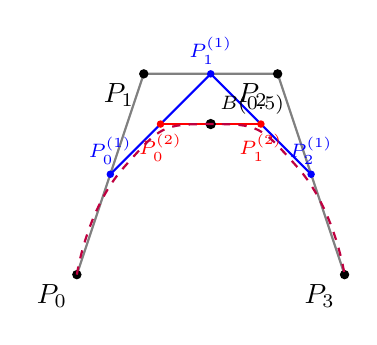
\begin{tikzpicture}[scale=0.85,>=stealth]
  % Control points
  \coordinate (P0) at (0,0);
  \coordinate (P1) at (1,3);
  \coordinate (P2) at (3,3);
  \coordinate (P3) at (4,0);

  % Level-1 points (t = 0.5 for visual clarity)
  \coordinate (Q0) at (0.5,1.5);
  \coordinate (Q1) at (2,3);
  \coordinate (Q2) at (3.5,1.5);

  % Level-2 points
  \coordinate (R0) at (1.25,2.25);
  \coordinate (R1) at (2.75,2.25);

  % Level-3 (B(0.5))
  \coordinate (B)  at (2,2.25);

  % Control polygon
  \draw[thick,gray] (P0)--(P1)--(P2)--(P3);
  \foreach \p/\l in {P0/$P_0$,P1/$P_1$,P2/$P_2$,P3/$P_3$}
     {\fill (\p) circle (2pt); \node[below left] at (\p) {\l};}

  % Level 1
  \draw[blue,thick] (Q0)--(Q1)--(Q2);
  \foreach \p/\l in {Q0/$P_0^{(1)}$,Q1/$P_1^{(1)}$,Q2/$P_2^{(1)}$}
     {\fill[blue] (\p) circle (1.6pt); \node[above,blue,font=\scriptsize] at (\p) {\l};}

  % Level 2
  \draw[red,thick] (R0)--(R1);
  \foreach \p/\l in {R0/$P_0^{(2)}$,R1/$P_1^{(2)}$}
     {\fill[red] (\p) circle (1.6pt); \node[below,red,font=\scriptsize] at (\p) {\l};}

  % B(t)
  \fill[black] (B) circle (2.2pt);
  \node[above right,font=\scriptsize] at (B) {$B(0.5)$};

  % Approximate curve sketch
  \draw[dashed,thick,purple] plot[smooth,tension=1] coordinates {(P0)(0.7,1.6)(2,2.25)(3.3,1.6)(P3)};
\end{tikzpicture}
\end{center}
\textbf{EN:} grey = control polygon; blue = level-1 polygon; red = level-2 segment; black = $B(t)$; dashed purple = the actual Bezier curve.

\switchcolumn

\subsection*{4.4* Hình minh hoạ De Casteljau}

\begin{center}
\textit{(Hình bên cột trái)}
\end{center}

\textbf{VI:} xám = control polygon gốc; xanh = đa giác mức 1 (lấy điểm chia $t$ trên mỗi cạnh); đỏ = đoạn mức 2; đen = điểm $B(t)$; tím nét đứt = đường cong Bezier thực sự.\\
Quan sát: các đoạn nối các điểm trung gian (đa giác xanh, đỏ) ngày càng tiệm cận đường cong; đa giác mức 1 thậm chí \emph{tiếp xúc} với curve tại $B(t)$ (đó là tiếp tuyến của curve tại $t$).

\medskip
\textbf{Tổng kết các mức:}
\begin{itemize}[leftmargin=*,nosep]
  \item Mức 0: $n{+}1$ điểm gốc $P_0,\dots,P_n$.
  \item Mức 1: $n$ điểm $P_i^{(1)}$ -- mỗi điểm chia một cạnh.
  \item Mức $k$: $n{+}1{-}k$ điểm.
  \item Mức $n$: \emph{một} điểm duy nhất $=B(t)$.
\end{itemize}
\textbf{Mẹo thi:} với $n=3$, kẻ \emph{tam giác De Casteljau} 4 cột $\to$ 3 cột $\to$ 2 cột $\to$ 1 cột. Khi $t=0.5$, các trọng số đối xứng nên tính nhanh hơn.

\switchcolumn*

% ---------------------------------------------------------------------
% 4.5  BEZIER SURFACE
% ---------------------------------------------------------------------
\subsection*{4.5 Bezier Surface (Tensor Product)}

A \textbf{Bezier surface (patch)} of bi-degree $(m,n)$ is defined by an $(m{+}1)\times(n{+}1)$ grid of control points $P_{ij}$ (the \emph{control net}):
\[
S(u,v)=\sum_{i=0}^{m}\sum_{j=0}^{n}B_i^{\,m}(u)\,B_j^{\,n}(v)\,P_{ij},
\quad (u,v)\in[0,1]^{2}.
\]

\textbf{Properties.}
\begin{itemize}[leftmargin=*,nosep]
  \item Corner interpolation: $S(0,0)=P_{00}$, $S(1,0)=P_{m0}$, $S(0,1)=P_{0n}$, $S(1,1)=P_{mn}$.
  \item Convex hull of the control net contains the patch.
  \item Affine invariance.
  \item \emph{Isoparametric curves} $u=u_0$ or $v=v_0$ are themselves Bezier curves of degree $n$ (resp.\ $m$).
  \item \emph{Boundary curves} are the four Bezier curves through the four edges of the control net.
  \item Tangent at corner $(0,0)$ along $u$: $S_u(0,0)=m(P_{10}-P_{00})$; along $v$: $S_v(0,0)=n(P_{01}-P_{00})$.
\end{itemize}

\textbf{Bicubic patch} ($m=n=3$): $4\times 4=16$ control points -- the workhorse of CAD/animation.

\begin{center}
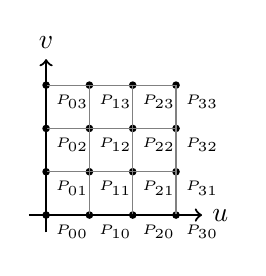
\begin{tikzpicture}[scale=0.55]
  \foreach \i in {0,1,2,3}{
    \foreach \j in {0,1,2,3}{
      \fill (\i,\j) circle (2.5pt);
      \node[font=\tiny,below right] at (\i,\j) {$P_{\i\j}$};
    }
  }
  % grid lines
  \foreach \i in {0,1,2,3}{ \draw[gray] (\i,0)--(\i,3); \draw[gray] (0,\i)--(3,\i); }
  \draw[->,thick] (-0.4,0)--(3.6,0) node[right]{$u$};
  \draw[->,thick] (0,-0.4)--(0,3.6) node[above]{$v$};
\end{tikzpicture}
\end{center}

\switchcolumn

\subsection*{4.5 Mặt Bezier (tích tensor)}

\textbf{Mặt (patch) Bezier} bậc $(m,n)$ được xác định bởi \emph{lưới control net} kích thước $(m{+}1){\times}(n{+}1)$:
\[
S(u,v)=\sum_{i=0}^{m}\sum_{j=0}^{n}B_i^{\,m}(u)B_j^{\,n}(v)P_{ij}.
\]

\textbf{Tính chất.}
\begin{itemize}[leftmargin=*,nosep]
  \item Nội suy 4 góc: $S(0,0)=P_{00}$, $S(1,0)=P_{m0}$, $S(0,1)=P_{0n}$, $S(1,1)=P_{mn}$.
  \item Nằm trong bao lồi của control net.
  \item Bất biến affine.
  \item \emph{Đường isoparametric} $u=u_0$ hoặc $v=v_0$ là đường cong Bezier bậc $n$ (hoặc $m$).
  \item \emph{4 đường biên} là 4 curve Bezier nằm trên 4 cạnh của control net.
  \item Tiếp tuyến tại góc $(0,0)$: $S_u=m(P_{10}-P_{00})$, $S_v=n(P_{01}-P_{00})$.
\end{itemize}

\textbf{Bicubic patch} ($m=n=3$): 16 control point -- dạng phổ biến nhất trong CAD/animation, mô phỏng vải, hoạt cảnh nhân vật...

\medskip
\textbf{Đường iso} có nghĩa là cố định một biến (vd $u=0.3$) rồi cho biến kia chạy. Đó vẫn là Bezier curve nên có thể áp dụng lại De Casteljau.

\switchcolumn*

% ---------------------------------------------------------------------
% 4.6  DE CASTELJAU ON SURFACES
% ---------------------------------------------------------------------
\subsection*{4.6 De Casteljau on Surfaces}

To compute $S(u,v)$ for a $(m{+}1)\times(n{+}1)$ control net:

\textbf{Method 1 (rows first).}
\begin{enumerate}[leftmargin=*,nosep]
  \item For each row $i=0,\dots,m$, run de Casteljau on $(P_{i0},\dots,P_{in})$ at parameter $v$ $\Rightarrow$ point $Q_i$.
  \item Run de Casteljau on $(Q_0,\dots,Q_m)$ at parameter $u$ $\Rightarrow$ $S(u,v)$.
\end{enumerate}
\textbf{Method 2 (columns first).} Swap the order: first reduce columns at $u$, then the resulting $(n{+}1)$ points at $v$. Same answer (tensor-product structure commutes).

\medskip
\textbf{Cost.} $O(m^{2}n+mn^{2})$ multiplications -- dominated by the smaller of the two passes. For bicubic ($m=n=3$): $4\times 6+4\times 6=48$ scalar lerps per coordinate $\approx$ trivial.

\begin{algorithm}[H]
\small
\DontPrintSemicolon
\KwIn{control net $P_{ij}$, $i{=}0..m,\,j{=}0..n$; $(u,v)$}
\For{$i\gets 0$ \KwTo $m$}{
   $Q_i \gets$ \textsc{DeCasteljau}$\bigl(P_{i0},\dots,P_{in};\,v\bigr)$\;
}
\Return \textsc{DeCasteljau}$(Q_0,\dots,Q_m;\,u)$\;
\caption{De Casteljau (surface, row-first)}
\end{algorithm}

\switchcolumn

\subsection*{4.6 De Casteljau cho mặt}

Để tính $S(u,v)$ trên control net $(m{+}1)\times(n{+}1)$:

\textbf{Cách 1 (theo hàng trước).}
\begin{enumerate}[leftmargin=*,nosep]
  \item Với mỗi hàng $i=0,\dots,m$: chạy De Casteljau trên $(P_{i0},\dots,P_{in})$ tại $v$, được điểm $Q_i$.
  \item Chạy De Casteljau trên $(Q_0,\dots,Q_m)$ tại $u$, được $S(u,v)$.
\end{enumerate}

\textbf{Cách 2 (theo cột trước).} Đảo thứ tự: rút cột trước (theo $u$), được $n{+}1$ điểm; rồi rút theo $v$. Kết quả \emph{giống nhau} do cấu trúc tensor.

\medskip
\textbf{Lựa chọn:} dùng \emph{cách hàng trước} nếu $m<n$ (ít vòng lặp ngoài), ngược lại dùng \emph{cách cột trước}. Với bicubic thì gần như tương đương.

\medskip
\textbf{Quan trọng cho thi:} vì cách nào cũng đúng, hãy chọn cách \emph{tận dụng được} các giá trị tròn (vd nếu $v=0.5$ thì giảm hàng trước cho dễ tính nhẩm).

\switchcolumn*

% ---------------------------------------------------------------------
% 4.7  WORKED EXAMPLE BEZIER SURFACE
% ---------------------------------------------------------------------
\subsection*{4.7 Worked Example --- Bezier Surface at $(u,v)=(0.5,0.5)$}

\textbf{Setup (biquadratic, $m=n=2$).} Use a $3\times 3$ control net (only the $z$-coordinate varies, $x=i$, $y=j$):
\[
P_{ij}=(i,\,j,\,h_{ij}),\qquad h=\begin{pmatrix}0&1&0\\1&3&1\\0&1&0\end{pmatrix},
\]
i.e.\ a small "tent" peaking at the centre. Compute $S(0.5,0.5)$.

\medskip
\textbf{Step 1 -- reduce each row at $v=0.5$ (quadratic De Casteljau).}

For row $i$, control points are $h_{i0},h_{i1},h_{i2}$; for $v=0.5$:
\[
Q_i = \tfrac14 h_{i0}+\tfrac12 h_{i1}+\tfrac14 h_{i2}.
\]
\begin{itemize}[leftmargin=*,nosep]
  \item Row 0: $Q_0^h=\tfrac14\cdot0+\tfrac12\cdot1+\tfrac14\cdot0=\tfrac12$. So $Q_0=(0,\,1,\,0.5)$.
  \item Row 1: $Q_1^h=\tfrac14\cdot1+\tfrac12\cdot3+\tfrac14\cdot1=\tfrac14+\tfrac32+\tfrac14=2$. So $Q_1=(1,\,1,\,2)$.
  \item Row 2: $Q_2^h=\tfrac14\cdot0+\tfrac12\cdot1+\tfrac14\cdot0=\tfrac12$. So $Q_2=(2,\,1,\,0.5)$.
\end{itemize}
(Note the $y$-coords come out as $1$ because $\tfrac14\cdot 0+\tfrac12\cdot 1+\tfrac14\cdot 2=1$.)

\textbf{Step 2 -- reduce $(Q_0,Q_1,Q_2)$ at $u=0.5$.}
\[
S=\tfrac14 Q_0+\tfrac12 Q_1+\tfrac14 Q_2.
\]
\begin{align*}
x &: \tfrac14\cdot 0+\tfrac12\cdot 1+\tfrac14\cdot 2 = 1,\\
y &: \tfrac14\cdot 1+\tfrac12\cdot 1+\tfrac14\cdot 1 = 1,\\
z &: \tfrac14\cdot 0.5+\tfrac12\cdot 2+\tfrac14\cdot 0.5 = 0.125+1+0.125=1.25.
\end{align*}
\[
\boxed{\,S(0.5,0.5)=(1,\,1,\,1.25)\,}.
\]

\medskip
\textbf{Sanity check (Bernstein direct).} For $n=m=2$ the Bernstein weights at $(0.5,0.5)$ are $(\tfrac14,\tfrac12,\tfrac14)\otimes(\tfrac14,\tfrac12,\tfrac14)$, the $z$-sum equals
\[
\tfrac{1}{16}\!\sum_{ij}w_{ij}h_{ij}\quad\text{with}\quad w=\begin{pmatrix}1&2&1\\2&4&2\\1&2&1\end{pmatrix}.
\]
$\sum w_{ij}h_{ij}=1\!\cdot\!0+2\!\cdot\!1+1\!\cdot\!0+2\!\cdot\!1+4\!\cdot\!3+2\!\cdot\!1+1\!\cdot\!0+2\!\cdot\!1+1\!\cdot\!0$
$=0+2+0+2+12+2+0+2+0=20$. So $z=20/16=1.25$. \checkmark

\switchcolumn

\subsection*{4.7 Ví dụ mặt Bezier tại $(u,v)=(0.5,0.5)$}

\textbf{Dữ liệu (bậc $2{\times}2$).} Lưới $3\times 3$, $x=i,y=j$, độ cao $h_{ij}$ như bảng:
\[
h=\begin{pmatrix}0&1&0\\1&3&1\\0&1&0\end{pmatrix}.
\]
Tính $S(0.5,0.5)$.

\textbf{Bước 1 -- giảm hàng tại $v=0.5$:}
trọng số bậc 2 là $(\tfrac14,\tfrac12,\tfrac14)$.
\begin{itemize}[leftmargin=*,nosep]
  \item Hàng 0: $z=\tfrac14(0)+\tfrac12(1)+\tfrac14(0)=0.5\Rightarrow Q_0=(0,1,0.5)$.
  \item Hàng 1: $z=\tfrac14(1)+\tfrac12(3)+\tfrac14(1)=2\Rightarrow Q_1=(1,1,2)$.
  \item Hàng 2: $z=0.5\Rightarrow Q_2=(2,1,0.5)$.
\end{itemize}

\textbf{Bước 2 -- giảm $(Q_0,Q_1,Q_2)$ tại $u=0.5$:}
\[
S=\tfrac14 Q_0+\tfrac12 Q_1+\tfrac14 Q_2 = (1,1,1.25).
\]
\[
\boxed{S(0.5,0.5)=(1,1,1.25)}.
\]

\textbf{Kiểm tra.} Theo Bernstein 2D, các trọng số là tích Kronecker
$(\tfrac14,\tfrac12,\tfrac14){\otimes}(\tfrac14,\tfrac12,\tfrac14)$, ma trận trọng số $\frac{1}{16}\begin{psmallmatrix}1&2&1\\2&4&2\\1&2&1\end{psmallmatrix}$. Nhân với ma trận $h$ rồi cộng tổng: $20/16=1.25$ \checkmark.

\medskip
\textbf{Mở rộng cho bicubic:} cũng tương tự nhưng có 4 hàng, mỗi hàng giảm theo De Casteljau bậc 3. Sau đó còn 4 điểm $Q_0..Q_3$, giảm tiếp 1 lần De Casteljau bậc 3 nữa $\to$ ra $S(u,v)$.

\switchcolumn*

% ---------------------------------------------------------------------
% 4.8  OTHER PARAMETRIC CURVES
% ---------------------------------------------------------------------
\subsection*{4.8 Other Parametric Curves (Context)}

\begin{itemize}[leftmargin=*,nosep]
  \item \textbf{Hermite}: defined by 2 endpoints $P_0,P_1$ and 2 tangents $T_0,T_1$. Cubic: $H(t)=h_{00}P_0+h_{10}T_0+h_{01}P_1+h_{11}T_1$ with the four Hermite basis polynomials $h_{00}=2t^3-3t^2+1$ etc.
  \item \textbf{Catmull--Rom}: an \emph{interpolating} spline through control points; tangent at $P_i$ is $\tfrac12(P_{i+1}-P_{i-1})$. Local control, $C^1$.
  \item \textbf{B-splines}: piecewise polynomials with \emph{knot vector}; only $k{+}1$ basis functions are non-zero on a span $\Rightarrow$ \emph{local control} (move one CP and only nearby curve changes). Bezier is the special case of a single non-uniform knot vector $\{0,\dots,0,1,\dots,1\}$.
  \item \textbf{NURBS} = Non-Uniform Rational B-Splines. Adds positive weights $w_i$:
        $C(t)=\dfrac{\sum w_i N_i^{p}(t) P_i}{\sum w_i N_i^{p}(t)}$. Can represent conics exactly (circle, ellipse).
\end{itemize}

\textbf{Comparison.}
\begin{center}\scriptsize
\begin{tabular}{@{}lcccc@{}}\toprule
 & Interp.? & Local ctrl? & Tangent ctl? & Conics? \\\midrule
Bezier         & endpoints only & no  & via $P_1,P_{n-1}$ & no \\
Hermite        & endpoints      & no  & yes (explicit)    & no \\
Catmull--Rom   & yes (all CP)   & yes & no (auto)         & no \\
B-spline       & no             & yes & no                & no \\
NURBS          & no (ctrl + $w$)& yes & no                & yes \\\bottomrule
\end{tabular}
\end{center}

\switchcolumn

\subsection*{4.8 Các loại đường cong tham số khác}

\begin{itemize}[leftmargin=*,nosep]
  \item \textbf{Hermite}: xác định bởi 2 điểm đầu mút + 2 tiếp tuyến. Bậc 3, hữu ích khi đã có thông tin tiếp tuyến.
  \item \textbf{Catmull--Rom}: spline \emph{nội suy} đi qua các control point; tiếp tuyến tại $P_i$ tự động tính $=\tfrac12(P_{i+1}-P_{i-1})$. Có local control, liên tục $C^1$.
  \item \textbf{B-spline}: đa thức piecewise, có \emph{knot vector}; mỗi hàm cơ sở chỉ ảnh hưởng cục bộ $\Rightarrow$ \emph{điều khiển địa phương}. Bezier là trường hợp đặc biệt với knot $\{0,\dots,0,1,\dots,1\}$.
  \item \textbf{NURBS} = B-spline \emph{hữu tỉ + không đều}; có trọng số $w_i$, biểu diễn được đường tròn / ellipse \emph{chính xác}, là chuẩn trong CAD.
\end{itemize}

\textbf{So sánh.}
\begin{center}\scriptsize
\begin{tabular}{@{}lcccc@{}}\toprule
 & Nội suy? & Local? & Tiếp tuyến? & Conic? \\\midrule
Bezier         & 2 đầu mút       & không & qua $P_1,P_{n-1}$ & không \\
Hermite        & 2 đầu mút       & không & có (tường minh)    & không \\
Catmull--Rom   & qua mọi CP      & có    & tự động            & không \\
B-spline       & không           & có    & không              & không \\
NURBS          & không (CP $+w$) & có    & không              & có \\\bottomrule
\end{tabular}
\end{center}

\switchcolumn*

% ---------------------------------------------------------------------
% 4.9  SUBDIVISION & DERIVATIVE & DEGREE ELEVATION
% ---------------------------------------------------------------------
\subsection*{4.9 Subdivision, Derivatives, Degree Elevation}

\textbf{Subdivision (free from De Casteljau).} Running de Casteljau at $t$ \emph{produces}, as a side product, the control polygons of the two halves of the curve:
\begin{align*}
\text{Left half:}\;& P_0^{(0)},\,P_0^{(1)},\,P_0^{(2)},\,\dots,\,P_0^{(n)},\\
\text{Right half:}\;& P_0^{(n)},\,P_1^{(n-1)},\,P_2^{(n-2)},\,\dots,\,P_n^{(0)}.
\end{align*}
The two halves together reproduce the original curve; this is the basis of \emph{adaptive rendering} (recursively subdivide until the polygon is "flat enough").

\textbf{Derivative.} The derivative of a degree-$n$ Bezier curve is itself a degree-$(n{-}1)$ Bezier curve on the \emph{forward differences}:
\[
B'(t)=n\sum_{i=0}^{n-1}B_i^{\,n-1}(t)\,(P_{i+1}-P_i).
\]
At endpoints: $B'(0)=n(P_1-P_0)$, $B'(1)=n(P_n-P_{n-1})$ (already noted).

\textbf{Degree elevation.} A degree-$n$ Bezier with points $P_0,\dots,P_n$ is also a degree-$(n{+}1)$ Bezier with $n{+}2$ points $P_i'$:
\[
P_i'=\tfrac{i}{n+1}P_{i-1}+\Bigl(1-\tfrac{i}{n+1}\Bigr)P_i,\quad i=0,\dots,n+1,
\]
(with $P_{-1}, P_{n+1}$ interpreted via the boundary cases $P_0'=P_0$, $P_{n+1}'=P_n$). Useful to make two Bezier patches/curves have matching degrees before joining.

\textbf{$C^1$ joining of two cubic Bezier curves} with control points $\{P_0,P_1,P_2,P_3\}$ then $\{Q_0,Q_1,Q_2,Q_3\}$:
need $Q_0=P_3$ ($C^0$) and $Q_1-Q_0 = P_3-P_2$ ($C^1$), i.e.\ $Q_1=2P_3-P_2$.

\switchcolumn

\subsection*{4.9 Phân chia, Đạo hàm, Nâng bậc}

\textbf{Phân chia (subdivision)} miễn phí từ De Casteljau. Khi chạy thuật toán tại $t$, các điểm trung gian \emph{tự sinh ra} 2 control polygon mới:
\[
\text{Trái: } P_0^{(0)},P_0^{(1)},\dots,P_0^{(n)};\quad
\text{Phải: } P_0^{(n)},P_1^{(n-1)},\dots,P_n^{(0)}.
\]
Hợp lại tái tạo đúng curve gốc -- là cơ sở để \emph{vẽ thích nghi} (đệ quy cho tới khi polygon đủ "phẳng" thì vẽ luôn các đoạn thẳng).

\textbf{Đạo hàm.} Đạo hàm của Bezier bậc $n$ là Bezier bậc $n{-}1$ trên \emph{sai phân}:
\[
B'(t)=n\sum_{i=0}^{n-1}B_i^{\,n-1}(t)(P_{i+1}-P_i).
\]
Ở đầu mút: $B'(0)=n(P_1-P_0)$, $B'(1)=n(P_n-P_{n-1})$.

\textbf{Nâng bậc (degree elevation).} Curve bậc $n$ có thể viết lại thành bậc $n{+}1$ với $n{+}2$ điểm
\[
P_i'=\tfrac{i}{n+1}P_{i-1}+\Bigl(1-\tfrac{i}{n+1}\Bigr)P_i.
\]
Hữu ích khi cần \emph{khớp bậc} 2 đoạn curve trước khi nối.

\textbf{Nối $C^1$ giữa 2 curve bậc 3} $\{P_i\}$ và $\{Q_i\}$:
$Q_0=P_3$ (cùng điểm), $Q_1=2P_3-P_2$ (cùng tiếp tuyến).

\switchcolumn*

% ---------------------------------------------------------------------
% 4.10  EXAM STRATEGIES
% ---------------------------------------------------------------------
\subsection*{4.10 Exam-Style Problems \& Strategies}

\begin{enumerate}[leftmargin=*,nosep]
  \item \emph{"Compute $B(t)$ at given $t$"} $\to$ De Casteljau (faster, fewer arithmetic mistakes than Bernstein for one $t$). Always lay out the triangle.
  \item \emph{"Compute $S(u,v)$"} $\to$ row-wise De Casteljau then column-wise. Decide order based on which $u$/$v$ is "nicer".
  \item \emph{"Subdivide at $t$"} $\to$ run De Casteljau, then read off the left/right control polygons (\S 4.9).
  \item \emph{"Tangent at endpoint"} $\to$ $B'(0)=n(P_1-P_0)$ or $B'(1)=n(P_n-P_{n-1})$.
  \item \emph{"Match $C^0/C^1$ between curves"} $\to$ shared endpoint + collinear adjacent control points with correct length ratio.
  \item \emph{"Verify a property"} (convex hull, partition of unity, etc.) $\to$ cite Bernstein property; show $\sum B_i^{n}(t)=1$ via $((1-t)+t)^n=1$.
  \item \emph{"Convert Bezier $\to$ monomial"} (rare): multiply out $\sum\binom{n}{i}(1-t)^{n-i}t^i P_i$ symbolically.
  \item \emph{"Pick t to minimise computation"}: $t=0,1,\tfrac12$ are easiest. $t=\tfrac13,\tfrac23$ keep things in thirds.
\end{enumerate}

\textbf{Common pitfalls.}
\begin{itemize}[leftmargin=*,nosep]
  \item Forgetting that weights are $(1-t)$ for the \emph{left} point and $t$ for the \emph{right} -- not the other way around.
  \item Using $\binom{n}{i}$ wrong (e.g.\ $\binom{3}{1}=3$ not $1$).
  \item In a surface problem, mixing up $u$/$v$ -- always label rows vs columns first.
  \item Forgetting that $B(0)=P_0$, $B(1)=P_n$ (not $P_1,\dots,P_{n-1}$).
\end{itemize}

\switchcolumn

\subsection*{4.10 Dạng bài thi \& Chiến thuật}

\begin{enumerate}[leftmargin=*,nosep]
  \item \emph{"Tính $B(t)$ tại $t$ cho trước"} $\to$ dùng De Casteljau (ít lỗi số học hơn Bernstein cho một giá trị $t$). Vẽ bảng tam giác rõ ràng.
  \item \emph{"Tính $S(u,v)$"} $\to$ giảm hàng theo $v$ trước, rồi giảm theo $u$ (hoặc ngược lại). Chọn thứ tự sao cho $t$ nào "đẹp" thì làm cuối.
  \item \emph{"Phân chia tại $t$"} $\to$ chạy De Casteljau, đọc 2 polygon ở 2 cạnh tam giác (\S 4.9).
  \item \emph{"Tiếp tuyến tại đầu mút"} $\to$ $B'(0)=n(P_1-P_0)$ hoặc $B'(1)=n(P_n-P_{n-1})$.
  \item \emph{"Nối $C^0/C^1$"} $\to$ trùng đầu mút + 3 điểm liền kề thẳng hàng, tỉ lệ độ dài hợp lý.
  \item \emph{"Chứng minh tính chất"} $\to$ trích dẫn Bernstein; tổng đa thức Bernstein $=((1-t)+t)^n=1$.
\end{enumerate}

\textbf{Lỗi hay gặp.}
\begin{itemize}[leftmargin=*,nosep]
  \item Lẫn trọng số: $(1-t)$ đi với điểm \emph{trái}, $t$ đi với điểm \emph{phải}.
  \item Sai $\binom{n}{i}$ -- nên chép luôn dòng Pascal trước khi tính.
  \item Trong bài surface, lẫn vai trò $u$/$v$ -- ghi rõ $i$ là chỉ số hàng, $j$ là cột.
  \item Nhớ $B(0)=P_0, B(1)=P_n$ -- KHÔNG đi qua các CP ở giữa.
\end{itemize}

\switchcolumn*

% ---------------------------------------------------------------------
% 4.11  BERNSTEIN TABLE
% ---------------------------------------------------------------------
\subsection*{4.11 Bernstein Coefficient Tables}

\textbf{Quadratic ($n=2$):} weights $((1-t)^2,\,2(1-t)t,\,t^2)$.
\begin{center}\small
\begin{tabular}{c|ccc|c}
$t$ & $B_0^2$ & $B_1^2$ & $B_2^2$ & sum \\\midrule
$0.25$ & $9/16=0.5625$ & $6/16=0.3750$ & $1/16=0.0625$ & 1\\
$0.50$ & $1/4=0.25$    & $1/2=0.50$    & $1/4=0.25$    & 1\\
$0.75$ & $1/16=0.0625$ & $6/16=0.3750$ & $9/16=0.5625$ & 1\\
\end{tabular}
\end{center}

\textbf{Cubic ($n=3$):} weights $((1-t)^3,\,3(1-t)^2t,\,3(1-t)t^2,\,t^3)$.
\begin{center}\small
\begin{tabular}{c|cccc|c}
$t$ & $B_0^3$ & $B_1^3$ & $B_2^3$ & $B_3^3$ & sum \\\midrule
$0.25$ & $27/64=0.421875$ & $27/64=0.421875$ & $9/64=0.140625$  & $1/64=0.015625$ & 1\\
$0.50$ & $1/8=0.125$      & $3/8=0.375$      & $3/8=0.375$      & $1/8=0.125$     & 1\\
$0.75$ & $1/64=0.015625$  & $9/64=0.140625$  & $27/64=0.421875$ & $27/64=0.421875$& 1\\
$1/3$  & $8/27\approx0.296$ & $12/27\approx0.444$ & $6/27\approx0.222$ & $1/27\approx0.037$ & 1\\
$2/3$  & $1/27$ & $6/27$ & $12/27$ & $8/27$ & 1\\
\end{tabular}
\end{center}

\textbf{Quartic ($n=4$) at $t=0.5$:}\\
$B^4=(\tfrac{1}{16},\tfrac{4}{16},\tfrac{6}{16},\tfrac{4}{16},\tfrac{1}{16})=(.0625,.25,.375,.25,.0625)$.

\textbf{Quintic ($n=5$) at $t=0.5$:}
$B^5=(1/32,\,5/32,\,10/32,\,10/32,\,5/32,\,1/32)$.

\textbf{Symmetry:} $B_i^n(t)=B_{n-i}^{\,n}(1-t)$ -- so the row at $t=0.75$ is the row at $t=0.25$ reversed (visible above).

\switchcolumn

\subsection*{4.11 Bảng tra hệ số Bernstein}

\textbf{Bậc 2:} trọng số $((1-t)^2,2(1-t)t,t^2)$.
\begin{center}\small
\begin{tabular}{c|ccc|c}
$t$ & $B_0^2$ & $B_1^2$ & $B_2^2$ & tổng \\\midrule
$0.25$ & $0.5625$ & $0.3750$ & $0.0625$ & 1\\
$0.50$ & $0.25$ & $0.50$ & $0.25$ & 1\\
$0.75$ & $0.0625$ & $0.3750$ & $0.5625$ & 1\\
\end{tabular}
\end{center}

\textbf{Bậc 3:}
\begin{center}\small
\begin{tabular}{c|cccc|c}
$t$ & $B_0^3$ & $B_1^3$ & $B_2^3$ & $B_3^3$ & tổng\\\midrule
$0.25$ & $0.421875$ & $0.421875$ & $0.140625$ & $0.015625$ & 1\\
$0.50$ & $0.125$ & $0.375$ & $0.375$ & $0.125$ & 1\\
$0.75$ & $0.015625$ & $0.140625$ & $0.421875$ & $0.421875$& 1\\
$1/3$  & $8/27$ & $12/27$ & $6/27$ & $1/27$ & 1\\
$2/3$  & $1/27$ & $6/27$ & $12/27$ & $8/27$ & 1\\
\end{tabular}
\end{center}

\textbf{Bậc 4 tại $t=0.5$:}
$(1,4,6,4,1)/16=(0.0625,0.25,0.375,0.25,0.0625)$.

\textbf{Bậc 5 tại $t=0.5$:}
$(1,5,10,10,5,1)/32$.

\textbf{Đối xứng:} $B_i^n(t)=B_{n-i}^{\,n}(1-t)$. Vì vậy hàng $t=0.75$ là hàng $t=0.25$ đảo chiều -- tiết kiệm thời gian khi tra bảng.

\textbf{Mẹo nhớ:} hệ số bậc $n$ là hàng $n$ của tam giác Pascal; phần $(1-t)^{n-i}t^i$ chính là "phép phối $n-i$ lần $1-t$ và $i$ lần $t$".

\switchcolumn*

% ---------------------------------------------------------------------
% 4.12  ONE-PAGE SUMMARY (FORMULA SHEET)
% ---------------------------------------------------------------------
\subsection*{4.12 One-Glance Formula Box}

\fbox{\parbox{0.95\columnwidth}{\small
\textbf{Bezier curve:}\;$B(t)=\sum_{i=0}^{n}\binom{n}{i}(1-t)^{n-i}t^{i}P_i$.\\[2pt]
\textbf{Bernstein:}\;$B_i^n(t)=\binom{n}{i}(1-t)^{n-i}t^i$,\;$\sum_i B_i^n(t)=1$.\\[2pt]
\textbf{De Casteljau:}\;$P_i^{(k)}=(1-t)P_i^{(k-1)}+tP_{i+1}^{(k-1)}$;\;$B(t)=P_0^{(n)}$.\\[2pt]
\textbf{Tangent:}\;$B'(0)=n(P_1-P_0)$,\;$B'(1)=n(P_n-P_{n-1})$.\\[2pt]
\textbf{Derivative curve:}\;$B'(t)=n\sum B_i^{n-1}(t)(P_{i+1}-P_i)$.\\[2pt]
\textbf{Degree elevation:}\;$P_i'=\tfrac{i}{n+1}P_{i-1}+(1-\tfrac{i}{n+1})P_i$.\\[2pt]
\textbf{Subdivision halves:}\\
\hspace*{6pt}left\;$=\{P_0^{(0)},P_0^{(1)},\dots,P_0^{(n)}\}$,\\
\hspace*{6pt}right\;$=\{P_0^{(n)},P_1^{(n-1)},\dots,P_n^{(0)}\}$.\\[2pt]
\textbf{Surface:}\;$S(u,v)=\sum_{i,j}B_i^m(u)B_j^n(v)P_{ij}$.\\[2pt]
\textbf{Surface eval:}\;rows-at-$v$ then column-at-$u$ (or vice-versa).\\[2pt]
\textbf{Corner:}\;$S(0,0)=P_{00}$, etc.\\[2pt]
\textbf{Surface tangents at $(0,0)$:}\;$S_u=m(P_{10}-P_{00})$,\;$S_v=n(P_{01}-P_{00})$.
}}

\switchcolumn

\subsection*{4.12 Khung công thức tóm tắt}

\fbox{\parbox{0.95\columnwidth}{\small
\textbf{Curve Bezier:}\;$B(t)=\sum\binom{n}{i}(1-t)^{n-i}t^{i}P_i$.\\[2pt]
\textbf{Bernstein:}\;$B_i^n=\binom{n}{i}(1-t)^{n-i}t^i$,\;tổng $=1$.\\[2pt]
\textbf{De Casteljau:}\;$P_i^{(k)}=(1-t)P_i^{(k-1)}+tP_{i+1}^{(k-1)}$.\\[2pt]
\textbf{Tiếp tuyến đầu mút:}\;$n(P_1-P_0)$ và $n(P_n-P_{n-1})$.\\[2pt]
\textbf{Đạo hàm:}\;$B'(t)=n\sum B_i^{n-1}(t)(P_{i+1}-P_i)$.\\[2pt]
\textbf{Nâng bậc:}\;$P_i'=\tfrac{i}{n+1}P_{i-1}+(1-\tfrac{i}{n+1})P_i$.\\[2pt]
\textbf{Phân chia:} polygon trái\;$\{P_0^{(0)},\dots,P_0^{(n)}\}$, phải\;$\{P_0^{(n)},\dots,P_n^{(0)}\}$.\\[2pt]
\textbf{Mặt:}\;$S(u,v)=\sum B_i^m(u)B_j^n(v)P_{ij}$.\\[2pt]
\textbf{Tính $S$:}\;giảm hàng tại $v$ rồi giảm cột tại $u$ (hoặc ngược lại).\\[2pt]
\textbf{Góc:}\;$S(0,0)=P_{00},\,S(1,0)=P_{m0},\,S(0,1)=P_{0n},\,S(1,1)=P_{mn}$.\\[2pt]
\textbf{Tiếp tuyến tại $(0,0)$:}\;$m(P_{10}-P_{00})$ và $n(P_{01}-P_{00})$.\\[2pt]
\textbf{Mẹo phòng thi:} luôn vẽ \emph{tam giác De Casteljau}, đánh dấu trọng số $1{-}t$ (trái) và $t$ (phải).
}}

\end{paracol}

% =====================================================================
% End of section 4
% =====================================================================
